\documentclass[aspectratio=169]{beamer}

\usetheme{Berlin}
\usecolortheme{metropolis}

\usepackage[portuguese]{babel}
\usepackage[utf8]{inputenc}
\usepackage[T1]{fontenc}
\usepackage{lmodern}
\usepackage{amsmath,amssymb}
\usepackage{xcolor}
\usepackage{booktabs}
\usepackage{graphicx}
\usepackage{tikz}
\usetikzlibrary{arrows.meta, positioning, shapes.geometric, fit, backgrounds}
\usepackage{appendixnumberbeamer}
\usepackage[round,authoryear]{natbib}
\bibliographystyle{plainnat}
\renewcommand{\bibfont}{\scriptsize}
\setlength{\bibsep}{3pt plus 0.3ex}
% Evita o aviso de \newblock indefinido do beamer com natbib
\providecommand{\newblock}{}

% Barra de navegação enxuta
\setbeamertemplate{navigation symbols}{}
\setbeamertemplate{caption}[numbered]
\setbeamercovered{transparent}

% Cores de destaque (usadas por \dado e pelos diagramas TikZ)
\definecolor{corDestaque}{RGB}{0,102,68}
\definecolor{corSuave}{RGB}{0,128,96}
% Blocos seguem o \usecolortheme escolhido (não sobrescrever aqui)

\newcommand{\dado}[1]{{\color{corDestaque}\textbf{#1}}}

\title{Data Warehouse para transparência orçamentária municipal: uma proposta para Juiz de Fora}
\author{Antônio Marcos Souza Pereira}
\institute{Departamento de Ciência da Computação \\ Universidade Federal de Juiz de Fora}
\date{Trabalho de Conclusão de Curso \\ Orientador: Prof. Dr. Victor Ströele de Andrade Menezes \\ 14 de julho de 2026}

\begin{document}

\shorthandoff{"}

{
% \setbeamertemplate{headline}{}
\begin{frame}
  \maketitle
\end{frame}
}

\begin{frame}{Sumário}
  \tableofcontents
\end{frame}

\AtBeginSection[]{
  \begin{frame}{Sumário}
    \tableofcontents[currentsection]
  \end{frame}
}

\section{Introdução}
\begin{frame}{Motivação}
  \begin{itemize}
    \item A Lei de Acesso à Informação~\citep{Lei:12.527:2011} consolidou o direito do cidadão aos dados do Estado e os portais da transparência passaram a publicar orçamento e finanças.
    \item Publicar dados não é o mesmo que prestar contas; a base legal existe, os portais estão no ar, mas a participação cidadã na fiscalização segue restrita.
  \end{itemize}
  \begin{block}{Três lacunas sustentam essa distância:}
    \begin{itemize}
      \item Social: linguagem contábil distante da experiência do cidadão.
      \item Técnica: dados dispersos, formatos heterogêneos, sem cruzamento.
      \item Pedagógica: falta instrumento que capacite a "ler o mundo" orçamentário~\citep{freire1967liberdade}.
    \end{itemize}
  \end{block}
\end{frame}

\begin{frame}{Problema de pesquisa}
  \begin{block}{Pergunta-problema}
    Como organizar, em um modelo dimensional, os dados publicados pelo Portal da Transparência de Juiz de Fora, de forma a reduzir as barreiras técnicas que afastam cidadãos não especialistas da execução orçamentária municipal?
  \end{block}
  \begin{columns}[T]
    \begin{column}{0.48\textwidth}
      Lado técnico
      \begin{itemize}\small
        \item Granularidade dos fatos e escolha das dimensões.
        \item Tratar inconsistências sem invisibilizá-las.
        \item Reprodutibilidade do \textit{pipeline}.
      \end{itemize}
    \end{column}
    \begin{column}{0.48\textwidth}
      Lado conceitual
      \begin{itemize}\small
        \item Em nome de quem se reorganiza o dado?
        \item Arquitetura de dados é uma escolha política.
      \end{itemize}
    \end{column}
  \end{columns}
\end{frame}

\begin{frame}{Objetivos}
  Objetivo geral: desenvolver um Data Warehouse para análise da execução orçamentária de Juiz de Fora, reorganizando dados em uma estrutura dimensional acessível à fiscalização cidadã.
  \begin{block}{Objetivos específicos}
    \begin{enumerate}\small
      \item Coletar e documentar receitas e despesas, identificando inconsistências nas fontes.
      \item Modelar dimensionalmente segundo Kimball (fatos e dimensões).
      \item Implementar processos de ETL (extração, limpeza, transformação, carga).
      \item Construir \textit{dashboards} interativos com linguagem acessível.
      \item Avaliar o painel frente ao portal em tarefas de fiscalização.
    \end{enumerate}
  \end{block}
\end{frame}

\section{Fundamentação}
\begin{frame}{Orçamento público}
  \begin{columns}[T]
    \begin{column}{0.52\textwidth}
      Instrumentos integrados
      \begin{itemize}\small
        \item PPA (4 anos) $\rightarrow$ LDO (prioridades) $\rightarrow$ LOA (ano).
      \end{itemize}
      \vspace{0.15cm}
      Estágios da despesa
      \begin{itemize}\small
        \item Empenho $\rightarrow$ Liquidação $\rightarrow$ Pagamento.
        \item Explica "restos a pagar" e o gap empenhado \textit{vs.} pago.
      \end{itemize}
    \end{column}
    \begin{column}{0.44\textwidth}
      \begin{block}{A barreira semântica}
        \small Manuais (MCASP, MTO) padronizam classificações para o emissor, não para o receptor. Termos como "elemento de despesa" e "funcional programática" afastam o cidadão.
      \end{block}
    \end{column}
  \end{columns}
\end{frame}

\begin{frame}{Controle social e a leitura freireana}
  \begin{itemize}
    \item Transparência $\neq$ \textit{accountability}: publicar é declarativo, mas prestar contas exige resposta e justificativa~\citep{pinho2009accountability}.
    \item Até observatórios sociais têm dificuldade para cruzar dados dos portais~\citep{marco2022transparencia}.
  \end{itemize}
  \begin{block}{Conscientização}
    A organização da informação não é neutra: ela define quem consegue ler os dados e, com isso, quem consegue fiscalizar.
  \end{block}
\end{frame}

\begin{frame}{Data Warehouse e modelagem dimensional~\citep{kimball2013data}}
  \begin{columns}[T]
    \begin{column}{0.5\textwidth}
      Propriedades do DW
      \begin{itemize}\small
        \item Orientado a assunto
        \item Integrado
        \item Não volátil
        \item Variável no tempo
      \end{itemize}
    \end{column}
    \begin{column}{0.5\textwidth}
      Esquema estrela
      \begin{itemize}\small
        \item Fatos: métricas (empenhado, liquidado, pago).
        \item Dimensões: contexto (tempo, órgão, função, fornecedor).
        \item Prioriza a usabilidade analítica sobre junções complexas.
      \end{itemize}
    \end{column}
  \end{columns}
  \vspace{0.2cm}
  \begin{block}{Tese central}
    Uma transparência efetiva precisa da estrutura de Kimball e do propósito de Freire.
  \end{block}
\end{frame}

\begin{frame}{Posicionamento frente à literatura}
  \small
  \begin{table}
    \centering
    \begin{tabular}{@{}p{3.4cm}p{3.6cm}p{3.6cm}@{}}
      \toprule
      \textbf{Dimensão} & \textbf{Literatura existente} & \textbf{Este trabalho} \\
      \midrule
      Esfera de governo & Capitais / federal & Municipal (JF) \\
      Integração receita/despesa & Parcial & Presente \\
      Reprodutibilidade & Código fechado & Aberto, instância pública \\
      \bottomrule
    \end{tabular}
  \end{table}
  \vspace{0.1cm}
  \footnotesize A literatura documenta amplamente as falhas dos portais, mas oferece poucas soluções técnicas concretas para interpretar os dados~\citep{melo2019proposta,teles2024panorama}.
\end{frame}

\section{Metodologia}
\begin{frame}{Design Science Research (DSR)~\citep{hevner2004,dresch2015}}
  \begin{itemize}
    \item O produto central é um artefato cuja relevância só se afere contra o problema que endereça.
    \item Ciclo iterativo em cinco fases:
  \end{itemize}
  \vspace{0.2cm}
  \begin{center}
  \footnotesize
  \begin{tikzpicture}[node distance=0.35cm, every node/.style={font=\footnotesize}]
    \tikzstyle{fase}=[rectangle, rounded corners=2pt, draw=corDestaque!70, thick,
      fill=corDestaque!10, minimum height=0.8cm, align=center, inner sep=4pt]
    \node[fase] (a) {Consciência\\do problema};
    \node[fase, right=of a] (b) {Sugestão};
    \node[fase, right=of b] (c) {Desenvolvimento};
    \node[fase, right=of c] (d) {Avaliação};
    \node[fase, right=of d] (e) {Conclusão};
    \draw[-{Stealth}, thick] (a)--(b);
    \draw[-{Stealth}, thick] (b)--(c);
    \draw[-{Stealth}, thick] (c)--(d);
    \draw[-{Stealth}, thick] (d)--(e);
  \end{tikzpicture}
  \end{center}
\end{frame}

\begin{frame}{Fontes de dados e inconsistências}
  \begin{columns}[T]
    \begin{column}{0.52\textwidth}
      Fontes
      \begin{itemize}\small
        \item Portal da Transparência PJF.
        \item Ementário da Receita Orçamentária.
        \item Classificação funcional da LOA.
      \end{itemize}
    \end{column}
    \begin{column}{0.46\textwidth}
      Avaliação funcional
      \begin{itemize}\small
        \item Portal \textit{vs.} painel: nº de passos, consolidação manual, mediação técnica.
      \end{itemize}
    \end{column}
  \end{columns}
  \vspace{0.2cm}
  \begin{block}{Postura metodológica}
    Inconsistências das fontes são tratadas como achado e não como ruído a ser corrigido silenciosamente.
  \end{block}
\end{frame}

\section{O Artefato}
\begin{frame}{Arquitetura em camadas}
  \begin{center}
  \begin{tikzpicture}[
      >={Stealth[length=2.5mm]},
      layer/.style={rectangle, rounded corners=3pt, draw=black!60, thick,
        minimum width=10.5cm, minimum height=0.82cm, align=center, inner sep=4pt, font=\small},
      arrow/.style={->, very thick, shorten >=1pt, shorten <=1pt}]
    \node[layer, fill=gray!8] (f) {\textbf{Fontes Públicas} \; \footnotesize Portal PJF (XLS) $\cdot$ STN (XLSX) $\cdot$ LOA (PDF/OCR)};
    \node[layer, fill=gray!16, below=0.28cm of f] (e) {\textbf{Extração} \; \footnotesize Dagster + Python + pandas $\rightarrow$ 6 \textit{assets}};
    \node[layer, fill=gray!24, below=0.28cm of e] (s) {\textbf{Staging} \; \footnotesize DuckDB + dbt: dedup, normalização};
    \node[layer, fill=corDestaque!25, below=0.28cm of s] (w) {\textbf{Warehouse} \; \footnotesize 10 dimensões + 3 fatos (Kimball)};
    \node[layer, fill=corDestaque!40, below=0.28cm of w] (c) {\textbf{Consumo} \; \footnotesize Streamlit + Plotly: 7 páginas, filtros globais};
    \draw[arrow] (f)--(e); \draw[arrow] (e)--(s); \draw[arrow] (s)--(w); \draw[arrow] (w)--(c);
  \end{tikzpicture}
  \end{center}
  \vspace{-0.15cm}
  \footnotesize Camadas desacopladas: mudança de \textit{layout} do portal fica confinada à
  extração/\textit{staging}.
\end{frame}

\begin{frame}{\textit{Stack} tecnológica}
  \centering
  \small
  \begin{tabular}{@{}lll@{}}
    \toprule
    \textbf{Componente} & \textbf{Papel} & \textbf{Camada} \\
    \midrule
    Dagster & Orquestração & Extração \\
    Python + pandas & Leitura/normalização de planilhas & Extração \\
    DuckDB & Banco analítico embarcado (OLAP colunar) & Staging / DW \\
    dbt & Modelagem dimensional em SQL & Staging / DW \\
    Streamlit + Plotly & \textit{Dashboards} interativos & Consumo \\
    \bottomrule
  \end{tabular}
  \vspace{0.3cm}
  \begin{block}{Critério de escolha}
    \small Reprodutibilidade local e baixa barreira de adoção: roda em máquina local, sem
    servidor, e publica no Streamlit Community Cloud.
  \end{block}
\end{frame}

\begin{frame}{Extração}
  \footnotesize Cada decisão nasceu de uma falha durante a implementação.
  \vspace{0.2cm}
  \begin{block}{Detecção dinâmica de cabeçalho}
    \small As planilhas de despesa não fixam a linha do cabeçalho. O parser varre até achar "Unidade Administrativa". Mudanças de \textit{layout} deixam de quebrar a carga.
  \end{block}
  \begin{block}{Quebra de \textit{layout} em 2025-05}
    \small Dois leitores coexistem (\texttt{pre2505} / \texttt{2505}): a escolha ocorre pela chave de partição e o histórico continua reprocessável.
  \end{block}
  \begin{block}{Classificação funcional da LOA (OCR)}
    \small PDFs escaneados $\rightarrow$ \texttt{pdftoppm} + Tesseract; o parser valida o exercício 2026.
  \end{block}
\end{frame}

\begin{frame}{Modelo dimensional}
  \begin{columns}[T]
    \begin{column}{0.46\textwidth}
      \textbf{Fatos}
      \begin{itemize}\scriptsize
        \item \texttt{fct\_despesa}: empenhado, liquidado, pago.
        \item \texttt{fct\_receita}: previsto e arrecadado no mês.
        \item \texttt{fct\_receita\_acumulada}: saldos anuais.
      \end{itemize}
      \vspace{0.1cm}
      \scriptsize
      Grão respeita o que a fonte publica: o relatório mensal consolidado, não a transação.
    \end{column}
    \begin{column}{0.52\textwidth}
      \centering
      \resizebox{\linewidth}{!}{%
      \begin{tikzpicture}[
          fact/.style={rectangle, rounded corners=2pt, draw=black!80, thick, fill=corDestaque!30,
            minimum width=1.7cm, minimum height=0.6cm, align=center, font=\tiny\ttfamily},
          dim/.style={rectangle, rounded corners=2pt, draw=black!50, fill=gray!10,
            minimum width=1.4cm, minimum height=0.45cm, align=center, font=\tiny\ttfamily},
          link/.style={-, thick, black!55}]
        \node[fact] (fd) at (0,0) {fct\_despesa};
        \node[dim] (d1) at (-2.3,1.3) {unidade};
        \node[dim] (d2) at (-2.6,0.2) {fornecedor};
        \node[dim] (d3) at (-2.3,-1.1) {funcional};
        \node[dim] (d4) at (0,-1.5) {natureza};
        \node[dim] (d5) at (0,1.5) {fonte};
        \node[dim] (d6) at (2.2,-1.1) {empenho};
        \foreach \d in {d1,d2,d3,d4,d5,d6}{\draw[link] (fd)--(\d);}
        \node[dim, fill=corDestaque!18, thick] (t) at (2.6,1.0) {dim\_tempo};
        \draw[link] (fd)--(t);
        \node[fact] (fr) at (4.6,0.6) {fct\_receita};
        \node[fact] (fra) at (4.6,-0.9) {fct\_rec\_acum};
        \node[dim, fill=corDestaque!18, thick] (nr) at (6.6,-0.15) {nat\_receita};
        \draw[link] (fr)--(t); \draw[link] (fra)--(t);
        \draw[link] (fr)--(nr); \draw[link] (fra)--(nr);
      \end{tikzpicture}%
      }
      \vspace{0.1cm}
      % \scriptsize \texttt{dim\_tempo} e \texttt{dim\_natureza\_receita} conformadas. \texttt{dim\_tempo} em \textit{role-playing} (empenho/liquidação).
    \end{column}
  \end{columns}
\end{frame}

\begin{frame}{Idempotência e qualidade de dados}
  \begin{columns}[T]
    \begin{column}{0.5\textwidth}
      \textbf{Idempotência}
      \begin{itemize}\small
        \item Reexecutar uma partição gera o mesmo estado final.
        \item Chaves substitutas por hash determinístico (MD5) sobre campos naturais.
      \end{itemize}
    \end{column}
    \begin{column}{0.5\textwidth}
      \textbf{Qualidade}
      \begin{itemize}\small
        \item Unicidade e não-nulidade de chaves.
        \item Integridade referencial fato--dimensão.
        \item Invariantes de domínio: acumulado não decrescente, a realizar = previsão $-$ arrecadado.
      \end{itemize}
    \end{column}
  \end{columns}
  \vspace{0.2cm}
%  \begin{block}{}
%    \small Em dados fiscais, falha silenciosa custa caro: um valor negativo por erro de \textit{parsing} pode virar conclusão errada sobre a execução orçamentária.
%  \end{block}
\end{frame}

\section{Resultados e Avaliação}
\begin{frame}{Camada de consumo}
  \begin{itemize}\small
    \item 5 páginas analíticas + Início + Glossário, sobre o mesmo DuckDB, com filtros globais.
  \end{itemize}
  \begin{center}
    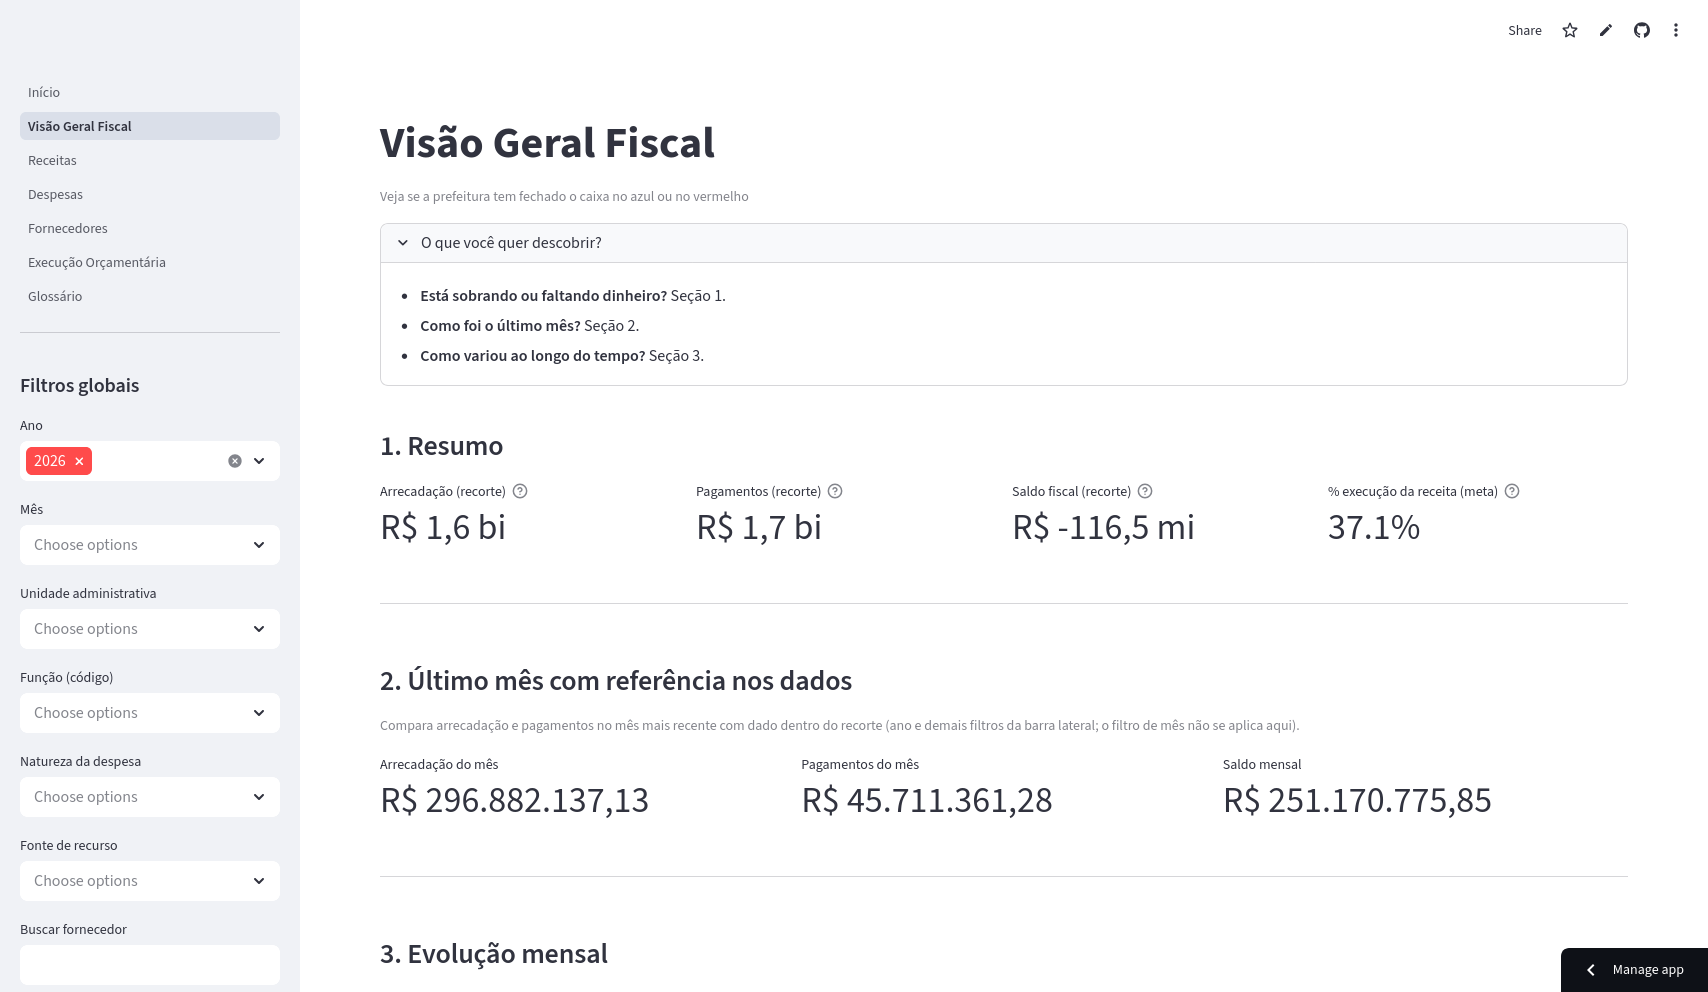
\includegraphics[width=0.82\textwidth,height=0.52\textheight,keepaspectratio]{figs/visao_geral_fiscal_1_2.png}
  \end{center}
  \footnotesize Visão Geral Fiscal: arrecadação, pagamentos, saldo fiscal e \% de execução da receita.
\end{frame}

\begin{frame}{Despesas}
  \begin{center}
    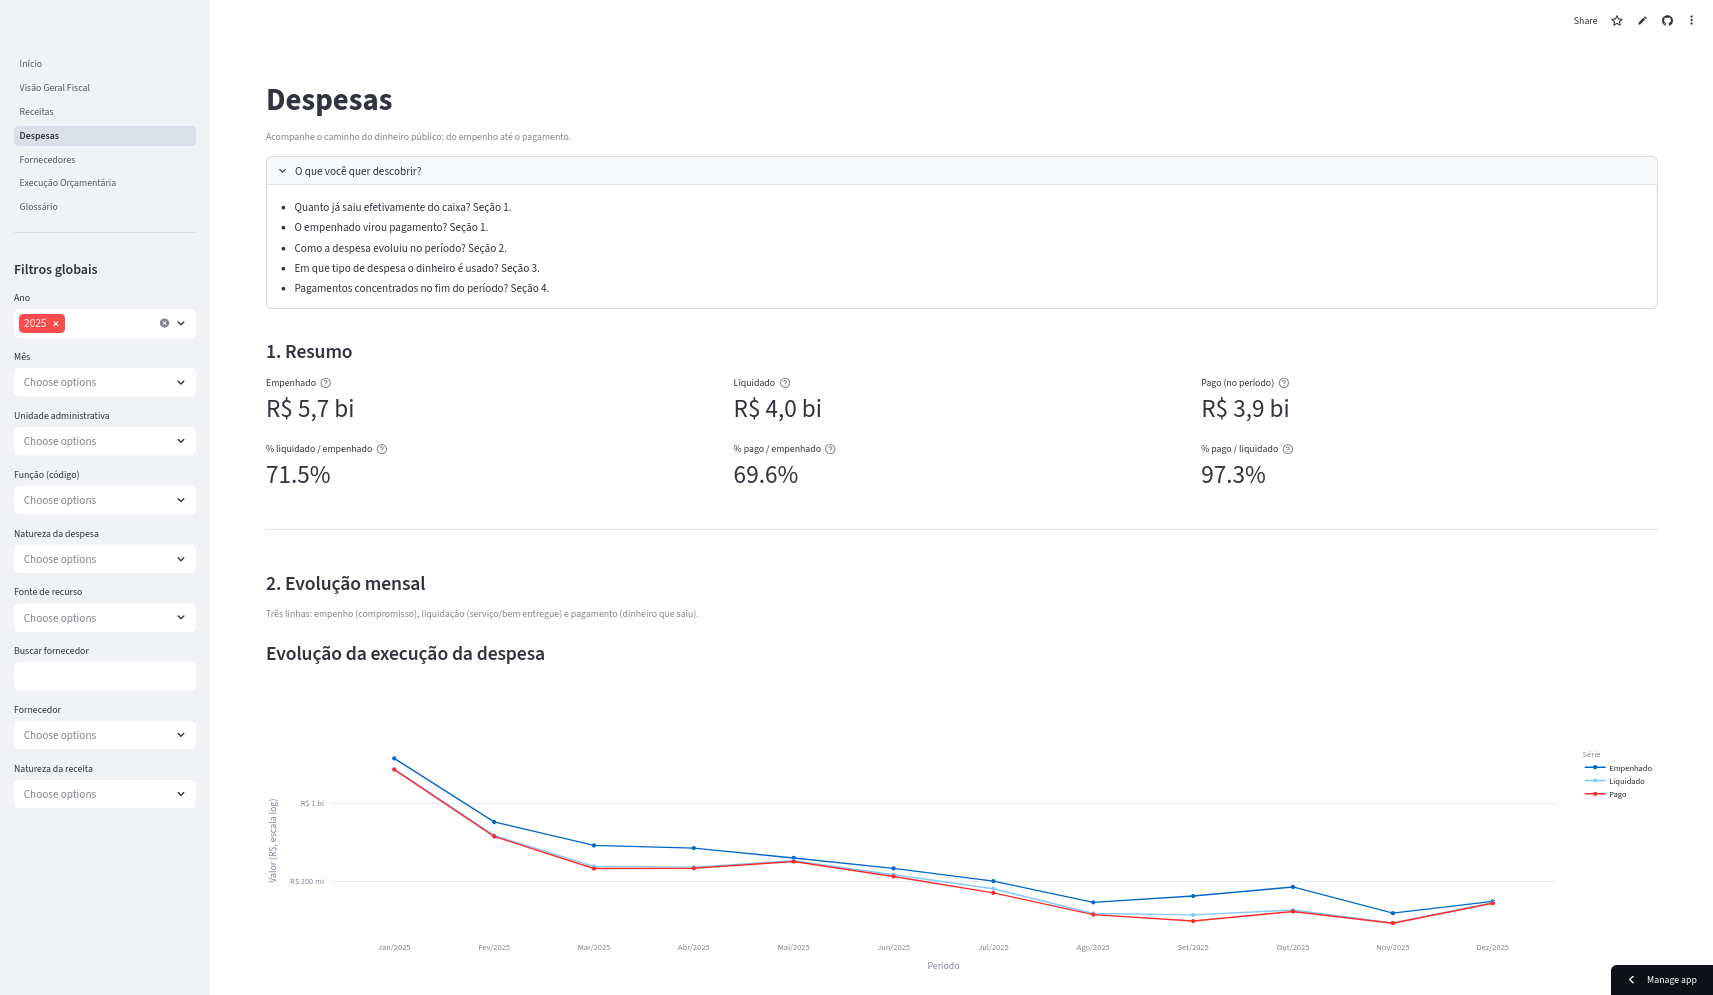
\includegraphics[width=0.88\textwidth,height=0.62\textheight,keepaspectratio]{figs/despesas_1_2.png}
  \end{center}
  \footnotesize No portal, comparar empenhado/liquidado/pago ao longo de anos exige consolidar vários arquivos mensais à mão. O painel devolve os indicadores em poucos cliques.
\end{frame}

\begin{frame}{Execução}
  \begin{center}
    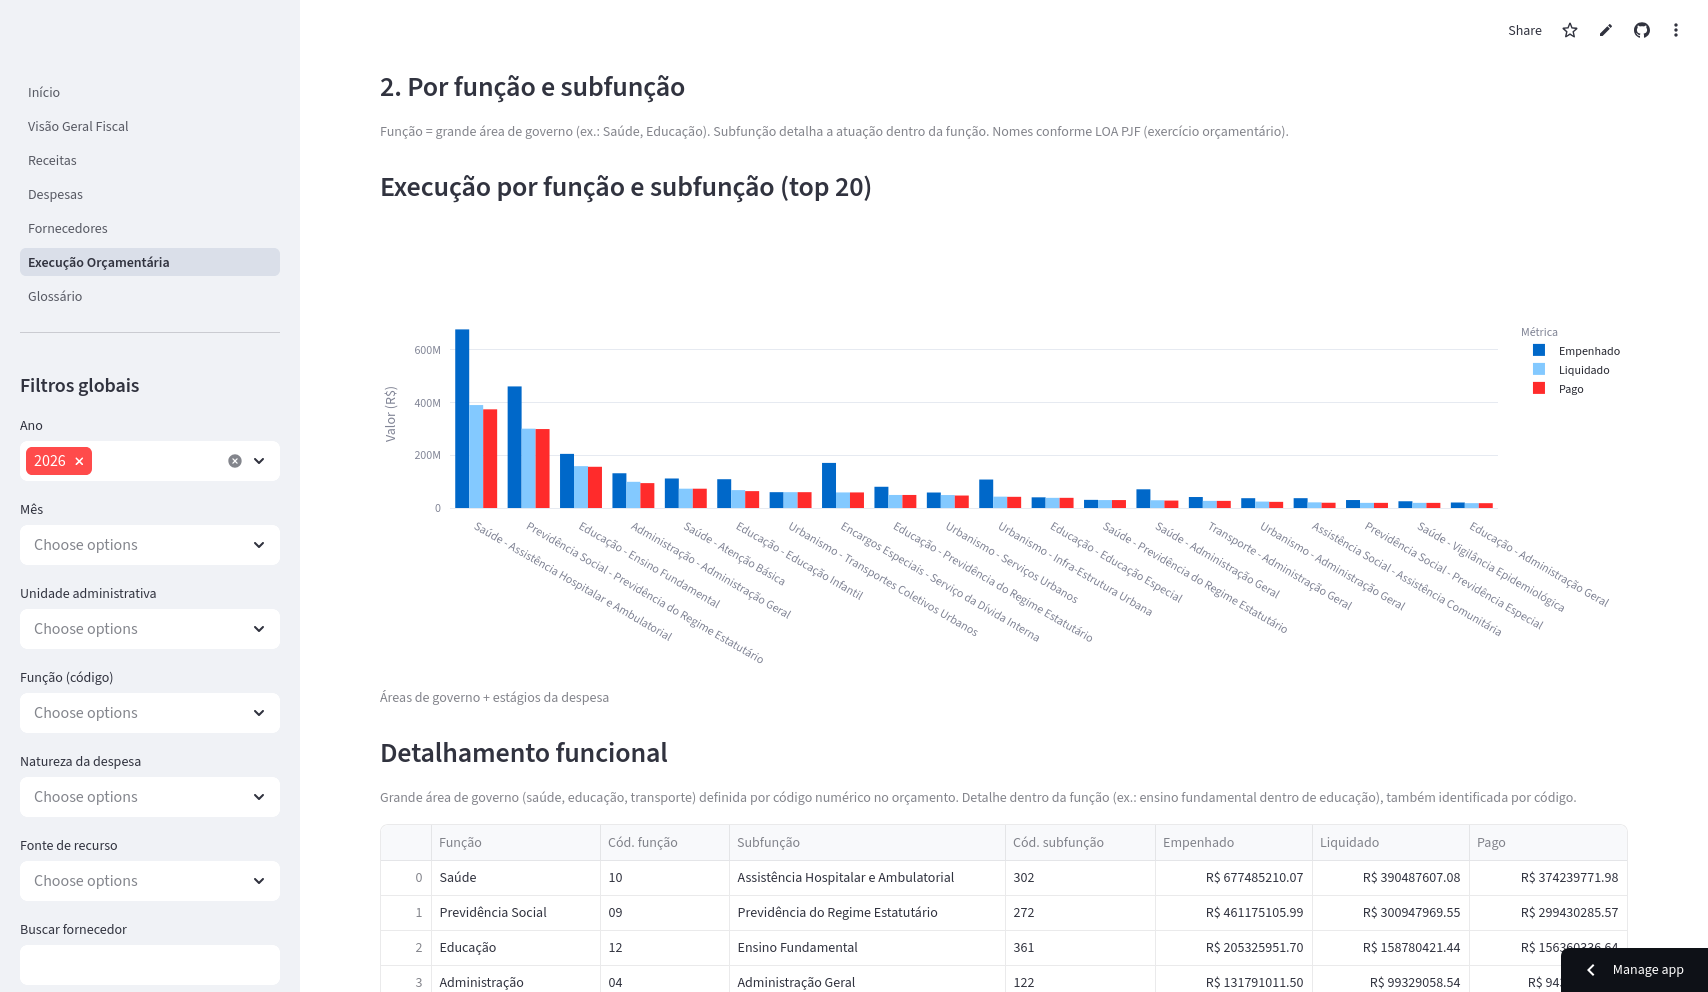
\includegraphics[width=0.82\textwidth,height=0.6\textheight,keepaspectratio]{figs/exec_2.png}
  \end{center}
  \footnotesize Responde, com ressalvas, à pergunta exemplar: \emph{"Quanto Juiz de Fora investiu em educação nos últimos anos?"} Não é preciso abrir doze planilhas anuais nem alinhar códigos à mão.
\end{frame}

\begin{frame}{Concentração de fornecedores}
  \begin{center}
    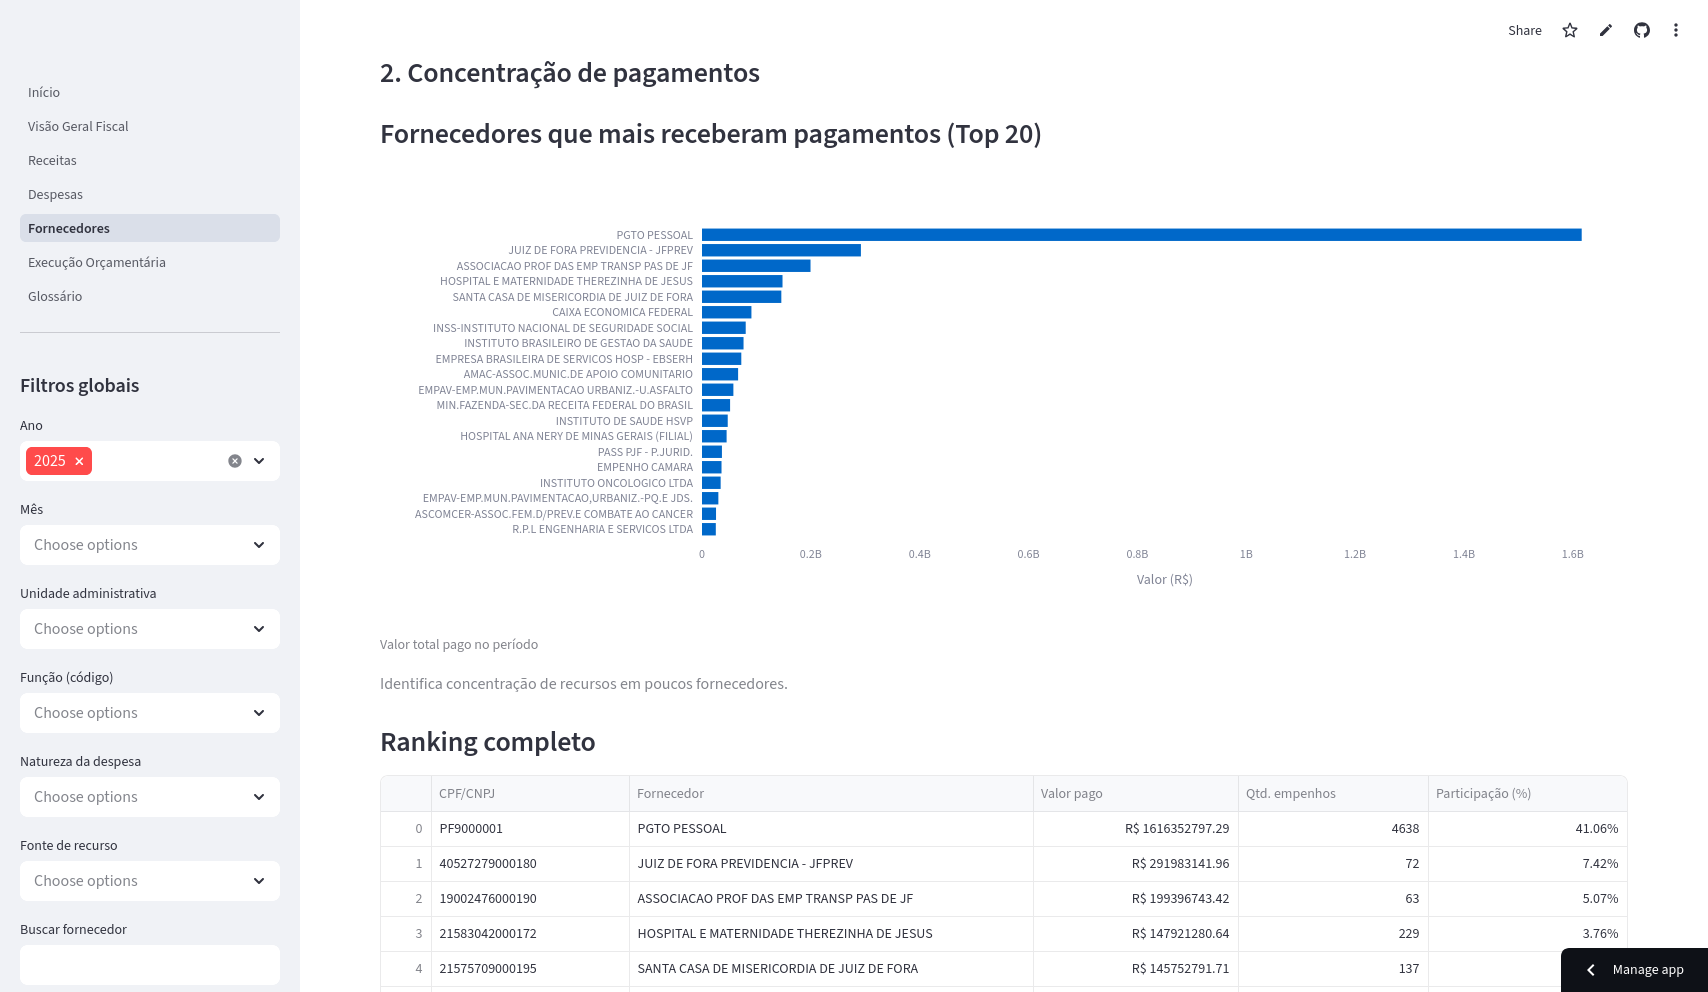
\includegraphics[width=0.78\textwidth,height=0.6\textheight,keepaspectratio]{figs/fornecedores_concentracao.png}
  \end{center}
  \footnotesize O indicador "\% nos 5 maiores" condensa a análise de concentração em um número legível e convida à pergunta: a dependência de poucos credores é compatível com o serviço?
\end{frame}

\begin{frame}{Receitas}
  \begin{center}
    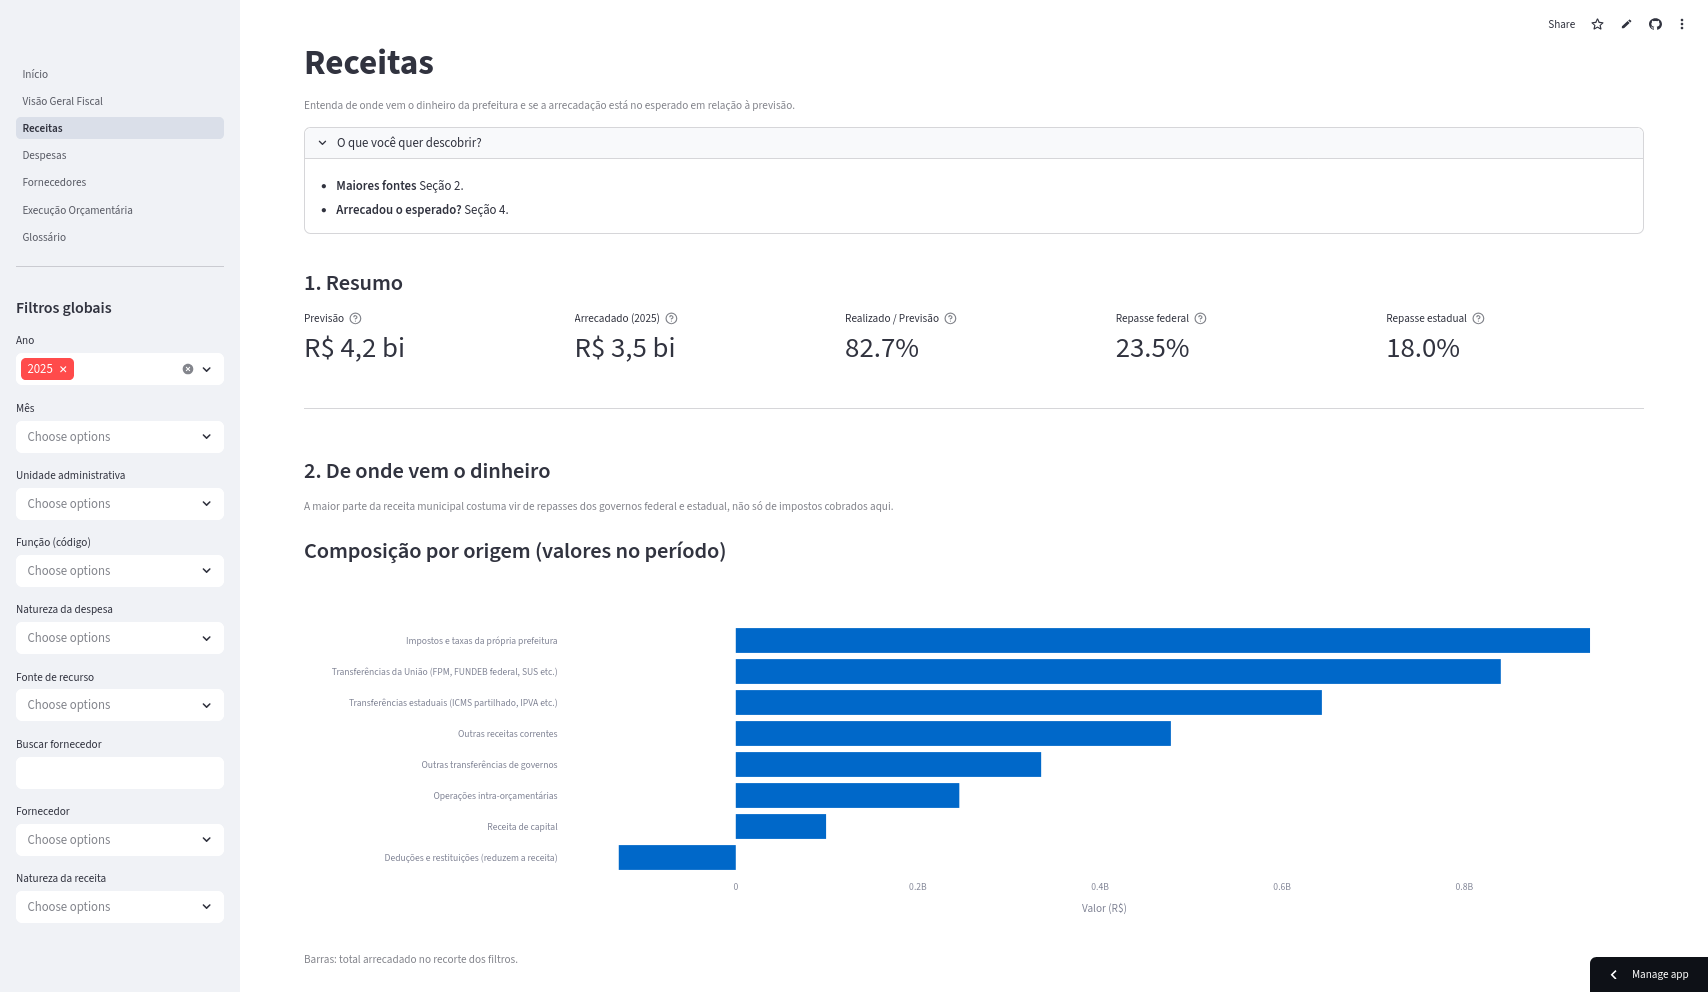
\includegraphics[width=0.82\textwidth,height=0.6\textheight,keepaspectratio]{figs/receitas.png}
  \end{center}
  \footnotesize Códigos MCASP agrupados por origem interpretável. Previsto \textit{vs.} realizado por natureza de receita, com descrições vindas do ementário da STN.
\end{frame}

\begin{frame}{O que os dados de Juiz de Fora revelam}
  \begin{block}{Dependência de transferências}
    \small Transferências correntes respondem por boa parte da arrecadação. Parte do orçamento da cidade depende de regras definidas fora do município.
  \end{block}
  \begin{block}{Distância entre empenho e pagamento}
    \small "Gastou" no sentido de empenho não coincide com "saiu do caixa".
  \end{block}
  \begin{block}{Legibilidade funcional incompleta}
    \small \textit{Fallbacks} de rótulo LOA (\textasciitilde 14\% dos pares função/subfunção) concentram-se em combinações de menor volume.
  \end{block}
\end{frame}

\begin{frame}{Avaliação}
  \scriptsize
  \begin{table}
    \centering
    \begin{tabular}{@{}p{3.9cm}p{4.3cm}p{3.6cm}@{}}
      \toprule
      \textbf{Pergunta de fiscalização} & \textbf{Portal da Transparência} & \textbf{Dashboard} \\
      \midrule
      Saldo arrecadação $\times$ pagamentos   &   Baixar planilhas, alinhar, somar à mão    &   Visão Geral Fiscal + filtrar ano \\
      Evolução empenhado/liquidado/pago   &   Vários arquivos, consolidar à mão   &   Página Despesas + gráfico único \\
      Pagamentos por função   &   Filtrar, somar, decodificar código    &   Tabela com rótulos LOA \\
      Maiores fornecedores    &   Exportar, ordenar, calcular \%  &   Indicador "\% nos 5 maiores" \\
      Previsão \textit{vs.} arrecadação   &   Reconciliar arquivos, interpretar códigos   &   Tabela com \% de realização \\
      Significado de "liquidação"   &   Buscar norma externa    &   Glossário + \textit{tooltips} \\
      \bottomrule
    \end{tabular}
  \end{table}
  \footnotesize O painel não cria dados novos, só reorganiza o que já foi publicado.
\end{frame}

\begin{frame}{Implicações para as três lacunas}
  \begin{itemize}
    \item Técnica: integrar receita e despesa, normalizar e expor séries temporais tira do usuário o trabalho de consolidação manual.
    \item Social: glossário e agrupamento por origem aproximam o MCASP do vocabulário público.
    \item Pedagógica: a estrutura por perguntas empurra o usuário a "ler o mundo", mas não substitui prestação de contas.
  \end{itemize}
\end{frame}

\section{Conclusão}
\begin{frame}{Contribuições}
  \begin{enumerate}\small
    \item Coleta e documentação de 6 fontes, com tratamento explícito de heterogeneidades.
    \item Modelagem Kimball com 10 dimensões e 3 fatos.
    \item ETL idempotente com Dagster + Python + DuckDB + dbt.
    \item Dashboards em Streamlit, publicados em instância pública. Avaliação: o painel reduz os passos manuais em todas as tarefas.
  \end{enumerate}
\end{frame}

\begin{frame}{Considerações finais}
  \begin{quote}
    "A leitura do mundo precede a leitura da palavra." (Paulo Freire)
  \end{quote}
  \vspace{0.2cm}
  \begin{itemize}
    \item O problema da transparência orçamentária municipal não é técnico: está na distância entre o que o portal publica e o que o cidadão precisa para fiscalizar.
    \item Reduzir essa distância é trabalho de arquitetura de dados e isso é uma decisão política.
    \item Conscientização orçamentária, para quem constrói \textit{data warehouses}, significa modelar o dado pensando em quem vai lê-lo.
  \end{itemize}
\end{frame}

\begin{frame}{Trabalhos futuros}
  \begin{enumerate}\small
    \item Integrar a dotação autorizada da LOA (indicadores de \% de execução sobre o autorizado).
    \item Desagregar a funcional programática em programa e ação.
    \item Capturar licitações e contratos como novos processos de negócio.
    \item Implementar SCD tipo 2 nas dimensões sujeitas a mudança histórica.
    \item Replicar o modelo em outro município de porte semelhante.
  \end{enumerate}
  \vspace{0.2cm}
\end{frame}

\appendix

\begin{frame}[allowframebreaks]{Referências}
  \bibliography{refs}
\end{frame}

{
\setbeamertemplate{headline}{}
\begin{frame}
  \centering {\Large \textbf{Obrigado!}}
\end{frame}
}

\end{document}
